\section{Komposition von Abbildungen}

\textbf{Definition (Komposition):}

Seien $f:D_f\rightarrow W_f$ und $g:D_g\rightarrow W_g$
zwei Abbildungen. Falls das Bild von $f$ im Definitionsbereich
von $g$ enthalten ist, also
\[
\operatorname{Bild}(f)\subseteq D_g,
\]
ist die Komposition $g\circ f$ auf ganz $D_f$ definiert durch
\[
g\circ f:D_f\rightarrow W_g,
\qquad (g\circ f)(x)=g(f(x)).
\]

Dabei wird zuerst $f$ und anschließend $g$ angewendet.
Es genügt insbesondere, wenn $W_f\subseteq D_g$ gilt.
Die schwächere Bedingung $\operatorname{Bild}(f)\subseteq D_g$
ist jedoch entscheidend, denn die Zielmenge $W_f$ kann
größer als das tatsächliche Bild sein.

% Die Abbildung verdeutlicht die Hintereinanderausführung.
\begin{center}
	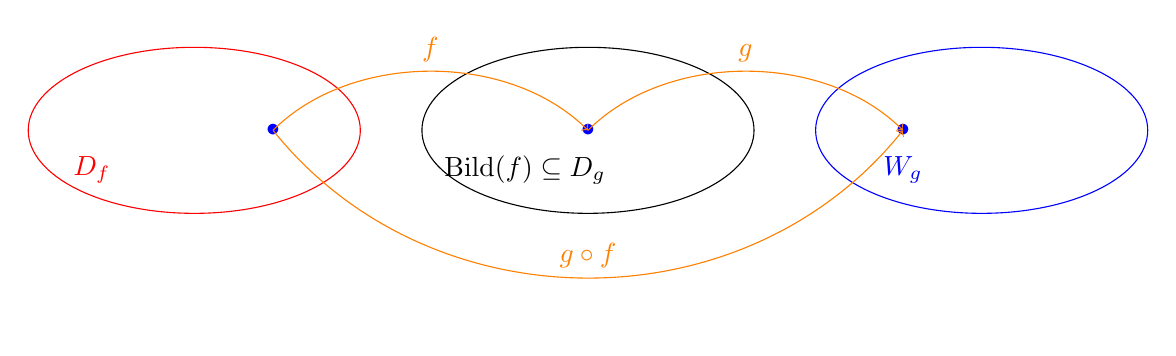
\begin{tikzpicture} 
		\draw[color=black] (5,0) ellipse (60pt and 30pt); 
		\draw[color=red] (0,0) ellipse (60pt and 30pt);
		\draw[color=blue] (10,0) ellipse (60pt and 30pt);
		%\draw[color=green] (5.5,0) ellipse (25pt and 15pt);
		
		\draw[color=black] (4.2,-.5) node { $\mathrm{Bild}(f)\subseteq\mathbb{D}_g$};
		\draw[color=red] (-1.3,-.5) node { $\mathbb{D}_f$};
		\draw[color=blue] (9,-0.5) node { $\mathbb{W}_g$};
		%\draw[color=green] (5.7,0) node { $\mathbb{V}$};
		\draw[color=blue,thick](1,0) node {$\bullet$};
		\draw[color=blue,thick](5,0) node {$\bullet$};
		\draw[color=blue,thick](9,0) node {$\bullet$};
		\draw[->,orange] (1, 0) .. controls(2, 1) and(4,1) .. node[above,sloped] {$f$}(5, 0);
		\draw[->,orange] (5, 0) .. controls(6, 1) and(8,1) .. node[above,sloped] {$g$}(9, 0);
		
		\draw[->,orange] (1, 0) .. controls(3, -2.5) and(7,-2.5) .. node[above,sloped] {$g\circ f$}(9, 0);
	\end{tikzpicture}
	
\end{center}

Ist $\operatorname{Bild}(f)$ nicht vollständig in $D_g$ enthalten,
kann $g\circ f$ dennoch auf der Teilmenge
\[
D_{g\circ f}=\{x\in D_f\mid f(x)\in D_g\}
\]
definiert werden. Diese Teilmenge kann auch leer sein.

\textbf{Beispiel:}

Seien
\[
\begin{aligned}
f:]0,1]&\rightarrow[1,\infty[,
& f(x)&=\frac1x,\\
g:[0,\infty[&\rightarrow[0,\infty[,
& g(x)&=\sqrt{x}.
\end{aligned}
\]

Untersuche die Kompositionen (i) $g\circ f$ und (ii) $f\circ g$.

\textbf{(i) Komposition $g\circ f$:}

Es gilt
\[
\operatorname{Bild}(f)=[1,\infty[\ \subseteq\ D_g=[0,\infty[.
\]
Damit ist $g\circ f$ auf dem gesamten Definitionsbereich
von $f$ definiert:
\[
\boxed{
(g\circ f)(x)=g\!\left(\frac1x\right)=\sqrt{\frac1x},
\qquad x\in\,]0,1].
}
\]
Also gilt
\[
g\circ f:\,]0,1]\rightarrow[0,\infty[.
\]
Tatsächlich ist das Bild von $g\circ f$ die Menge $[1,\infty[$.

\textbf{(ii) Komposition $f\circ g$:}

Hier gilt
\[
\operatorname{Bild}(g)=[0,\infty[\ \nsubseteq\ D_f=\,]0,1].
\]
Daher ist $f\circ g$ \emph{nicht auf ganz} $D_g=[0,\infty[$
definiert. Dennoch kann die Komposition auf einer geeigneten
Teilmenge gebildet werden. Aus
\[
\sqrt{x}\in\,]0,1]
\quad\Longleftrightarrow\quad
0<x\leq1
\]
folgt der zulässige Definitionsbereich $D_{f\circ g}=\,]0,1]$.
Somit gilt
\[
\boxed{
(f\circ g)(x)=f(\sqrt{x})=\frac1{\sqrt{x}},
\qquad x\in\,]0,1].
}
\]
Das Bild der eingeschränkten Komposition ist $[1,\infty[$.

\subsection{Aufgabe zur Komposition von Abbildungen}

\textbf{Aufgabe:}

Betrachte die Abbildungen
\[
\begin{aligned}
f:\mathbb R&\rightarrow\mathbb R,
&f(x)&=1+x^4,\\
h:\mathbb R&\rightarrow\mathbb R,
&h(x)&=1+x^3.
\end{aligned}
\]
Untersuche:

(i) Existiert eine Funktion $g$, sodass $h=g\circ f$
für alle $x\in\mathbb R$ gilt?

(ii) Existiert eine reellwertige Funktion $g$, sodass
$h=f\circ g$ für alle $x\in\mathbb R$ gilt?

\textbf{Lösung zu (i):}

Angenommen, eine Funktion $g$ mit $h=g\circ f$
existiert auf ganz $\mathbb R$. Dann müsste gelten:
\[
g(1+x^4)=1+x^3
\qquad\text{für alle }x\in\mathbb R.
\]
Da $f(1)=f(-1)=2$, folgt einerseits
\[
g(2)=h(1)=2,
\]
andererseits aber
\[
g(2)=h(-1)=0.
\]
Dies ist ein Widerspruch. Daher existiert \emph{keine}
solche Funktion $g$ auf ganz $\mathbb R$.

\textbf{Warum funktioniert der zunächst naheliegende Ansatz nicht?}

Für $t\geq1$ könnte man setzen:
\[
g(t)=1+\bigl(\sqrt[4]{t-1}\bigr)^3.
\]
Dann erhält man jedoch
\[
(g\circ f)(x)=1+\bigl(\sqrt[4]{x^4}\bigr)^3
=1+|x|^3.
\]
Dies stimmt nur für $x\geq0$ mit $h(x)=1+x^3$ überein.
Der Ansatz funktioniert also, wenn $f$ und $h$ auf
$[0,\infty[$ eingeschränkt werden; dann kann man
$g:[1,\infty[\rightarrow[1,\infty[$ wie oben definieren.

\textbf{Lösung zu (ii):}

Angenommen, es existiert eine reellwertige Funktion $g$
mit $h=f\circ g$ auf ganz $\mathbb R$. Dann müsste gelten:
\[
1+x^3=f(g(x))=1+(g(x))^4.
\]
Für jedes reelle $g(x)$ gilt $(g(x))^4\geq0$.
Somit wäre $h(x)\geq1$ für alle $x\in\mathbb R$.
Für $x=-1$ gilt jedoch $h(-1)=0$. Dies ist ein Widerspruch.
Daher existiert auch hier \emph{keine} solche Funktion $g$
auf ganz $\mathbb R$.

Für $x\geq0$ ist hingegen
\[
g(x)=x^{3/4}
\]
reell definiert, und es gilt
\[
(f\circ g)(x)=1+\bigl(x^{3/4}\bigr)^4
=1+x^3=h(x).
\]
Auf dem eingeschränkten Definitionsbereich $[0,\infty[$
ist eine solche Darstellung also möglich.

\textbf{Merke:}

Bei Kompositionen sind die Definitionsbereiche entscheidend.
Außerdem ist bei geraden Wurzeln zu beachten:
\[
\sqrt[4]{x^4}=|x|.
\]
